\documentclass[conference]{IEEEtran}
\IEEEoverridecommandlockouts
\usepackage{cite}
\usepackage{amsmath,amssymb,amsfonts}
\usepackage{newtxtext,newtxmath}
\usepackage{graphicx}
\usepackage{booktabs}
\usepackage{multirow}
\usepackage{algorithm}
\usepackage{algpseudocode}
\usepackage{textcomp}
\usepackage{xcolor}
\usepackage[hyphens]{url}
\def\BibTeX{{\rm B\kern-.05em{\sc i\kern-.025em b}\kern-.08em T\kern-.1667em\lower.7ex\hbox{E}\kern-.125emX}}
\newcommand{\Ledger}{\mathcal{L}}
\newcommand{\Obs}{\Omega}
\raggedbottom
\begin{document}

\title{Hub-less Cross-Honeypot Threat Intelligence:\\Federated IOC Corroboration on a Shared Ledger}

\author{
\IEEEauthorblockN{Suhas Reddy Annem\textsuperscript{1}, Sisir Reddy Nellore\textsuperscript{2}, Radhika G\textsuperscript{3}}
\IEEEauthorblockA{\textit{Department of Computer Science and Engineering}\\
\textit{Amrita School of Computing, Coimbatore}\\
\textit{Amrita Vishwa Vidyapeetham, India}\\
cb.sc.u4cse24503@cb.students.amrita.edu\textsuperscript{1}, cb.sc.u4cse23129@cb.students.amrita.edu\textsuperscript{2}, g\_radhika@cb.amrita.edu\textsuperscript{3}}
}

\maketitle

\begin{abstract}
Honeypots run by different organizations observe fragments of the same attack campaigns, but correlating those fragments normally requires a central threat-intelligence server that every sensor must trust and depend on. This paper evaluates a design with no such server. Each honeypot node hashes the indicators of compromise (IOCs) it observes and writes the digest, tagged with its identity, to a shared append-only ledger; any reader recovers provenance and cross-node corroboration from ledger history alone. We formalize the scheme, derive its gas and bootstrap cost models, and add a commit--reveal extension against an \emph{echo} adversary who re-anchors other nodes' digests to fabricate corroboration. All measurements are taken on a live Ethereum-compatible chain with up to 16 concurrent writers, five repetitions per configuration, and a measured centralized-hub baseline. Throughput saturates near 255 events/s by eight writers, with a median anchor latency of 11.74\,ms, against 1,737 events/s for the hub. Measured gas matches the EIP-2028 calldata model exactly (22,120 gas per IOC) and falls to 337 with 64-way Merkle batching; a new node rebuilds the global view at 3.01\,ms per block ($R^2=0.998$). When IOCs vary per target, campaign-level $F_1$ ranges from 0.15 to 0.89 across four keying functions, and exact-record hashing recovers only 27.5\% of multi-target campaigns. The echo adversary falsely corroborates 100\% of single-node digests under the plain scheme and 0\% under commit--reveal, at 2.0$\times$ the gas. Post-hoc tampering with a node's local log is detected in 500/500 trials with no false positives on 500 controls.
\end{abstract}

\begin{IEEEkeywords}
threat intelligence sharing, honeypot, blockchain, indicators of compromise, commit--reveal, Sybil attack, decentralized coordination
\end{IEEEkeywords}

\section{Introduction}

Attack campaigns are rarely confined to one target. Credential-stuffing botnets, mass scanners, and operators reusing an exploit kit produce related indicators against every honeypot they reach. A single decoy, however well instrumented, records only its own slice. The established remedy is centralization: an organization operates a threat-intelligence platform, every sensor reports into it, and the platform performs correlation. MISP~\cite{ref1} and the STIX/TAXII standards~\cite{ref2,ref3} formalize this arrangement with a common data model and a client--server transport.

Centralization removes fragmentation but introduces a dependency. The aggregator is a single point of trust, since every contributor must accept that it will neither lose nor alter nor withhold what it receives; it is a single point of failure, since correlation stops when it is unavailable; and it is an attractive target, since compromising one host blinds the whole sensor network. This dependency is particularly awkward in a honeypot deployment, where the decoys are built to be attacked but the correlating host is exposed to the same adversary without the same expectation.

This paper determines which functions of a centralized aggregator can be preserved when the aggregator is replaced by a shared append-only ledger to which every node writes tagged hashes. Prior blockchain-based CTI designs generally place logic on-chain (reputation contracts, access policy, membership enrollment), which enlarges the trusted surface and complicates evaluation~\cite{ref4,ref5,ref6,ref7}. We evaluate the opposite end of the design space: no contract, no registry, no inter-node communication, and a fixed decoding rule that any reader applies to raw transaction history.

The contributions are as follows.
\begin{enumerate}
\item A formal statement of the hub-less corroboration scheme (Section~\ref{sec:model}), including the observer map, the corroboration predicate, and a tamper-detection predicate for a node's local log, together with closed-form gas and bootstrap cost models that are checked against measurement.
\item A commit--reveal extension (Section~\ref{sec:cr}) that prevents an echo adversary from inflating corroboration by re-anchoring digests it reads from the ledger, and a quantification of what the extension costs in gas and in corroboration window.
\item An experimental evaluation on a live Ethereum-compatible chain with 1 to 16 concurrent writers, five repetitions per configuration and 95\% confidence intervals: scaling and tail latency, gas per IOC under two tag encodings and Merkle batching, bootstrap cost as a function of history length, campaign-level corroboration accuracy under four keying functions when IOCs vary per target, Sybil and echo adversaries, tamper detection with a false-positive control, and a measured centralized-hub baseline including an injected outage (Sections~\ref{sec:setup}--\ref{sec:results}).
\item A statement of the conditions under which the local-chain results transfer to a distributed deployment, and of the attacks the scheme does not address (Section~\ref{sec:discussion}).
\end{enumerate}

\section{Related Work}

\subsection{Centralized and federated CTI platforms}
MISP~\cite{ref1} supports a federated topology in which instances synchronize, but each instance is an administered server, synchronization relationships are configured pairwise, and a new participant must be admitted before it receives anything. STIX~\cite{ref2} and TAXII~\cite{ref3} standardize the indicator data model and the client--server transport; in a TAXII deployment, clients push to and pull from named collections on servers they must be configured with and authorized at. A user study of MISP by Stojkovski et al.~\cite{ref8} identifies the establishment and maintenance of trust relationships as a persistent source of friction. The scheme evaluated here has no server to be introduced to and no relationship to configure: all nodes write to one ledger, and any reader reads it.

\subsection{Blockchain-based CTI sharing}
Ruggiero and Bonomi~\cite{ref4} review requirements and residual threats for ledger-based CTI exchange. TRADE~\cite{ref5} is a peer-to-peer exchange in which the producer controls dissemination; TrustShare~\cite{ref6} combines on-chain records with access-control machinery; Dunnett et al.\ survey the challenges~\cite{ref11} and propose a verifiable, differential sharing framework~\cite{ref7}; BFLS~\cite{ref9} shares detection models rather than indicators through federated learning; Tariq et al.~\cite{ref12} survey the wider space. These systems place policy, reputation, or coordination logic on-chain. The present work is deliberately minimal (tagged hashes only) so that the properties of the substrate can be measured without confounding them with contract behavior. Table~\ref{tab:compare} summarizes the positioning.

\subsection{Byzantine agreement and honeypot sensing}
Agreement among mutually distrusting writers is the Byzantine generals problem~\cite{ref13}; the base chain's consensus solves it and the scheme inherits that guarantee rather than re-implementing it. Honeypots have long been used as sensors, on the premise that any traffic they receive is unsolicited~\cite{ref14,ref15}; Vetterl and Clayton showed that low- and medium-interaction decoys are fingerprintable at Internet scale~\cite{ref16}, which is one reason to correlate many sensors rather than rely on one. Otoum et al.~\cite{ref10} coordinate adaptive IoT honeypots through a trust-aware ledger in which nodes read and write contract state; here nodes exchange nothing and consult no trust score.

\begin{table}[!t]
\caption{Positioning against prior CTI-sharing designs.}
\label{tab:compare}
\centering
\scriptsize
\setlength{\tabcolsep}{3pt}
\begin{tabular}{@{}lcccc@{}}
\toprule
System & \shortstack{No trusted\\coordinator} & \shortstack{Bootstrap from\\ledger alone} & \shortstack{On-chain\\logic} & \shortstack{Adversary and\\cost measured} \\
\midrule
MISP federation~\cite{ref1,ref8} & -- & -- & n/a & -- \\
STIX/TAXII~\cite{ref2,ref3} & -- & -- & n/a & -- \\
TRADE~\cite{ref5}, TrustShare~\cite{ref6} & $\bullet$ & -- & contracts & -- \\
Dunnett et al.~\cite{ref7}, BFLS~\cite{ref9} & $\bullet$ & -- & contracts & -- \\
Otoum et al.~\cite{ref10} & $\bullet$ & -- & trust state & -- \\
This work & $\bullet$ & $\bullet$ & none & $\bullet$ \\
\bottomrule
\end{tabular}
\end{table}

\section{System Model and Problem Statement}
\label{sec:model}

\subsection{Entities and notation}
Let $\mathcal{P}=\{P_1,\dots,P_N\}$ be independently operated honeypot nodes. Node $P_i$ observes a stream of records $r\in\mathcal{R}$; in our implementation $r=(\mathit{src},\mathit{payload})$, the attacker source address and the captured payload string. Nodes hold no assumptions about one another: they need not be mutually reachable, they never exchange messages, and each is identified only by a signing key that authorizes transactions from account $a_i$ on a shared ledger $\Ledger$. The ledger is an ordered sequence of transactions; $\mathrm{ht}(\tau)$ denotes the block height at which transaction $\tau$ is included. $H$ denotes SHA-256~\cite{ref17}.

A \emph{keying function} $\kappa:\mathcal{R}\to\{0,1\}^*$ selects and normalizes the fields of a record that define ``the same indicator''. The digest of a record under $\kappa$ is $h=H(\kappa(r))$. Section~\ref{sec:keys} defines the four keying functions evaluated.

\subsection{Anchoring and the observer map}
To anchor a record, $P_i$ submits a self-transfer transaction from $a_i$ whose calldata carries the tag $\langle i,h\rangle$. No raw indicator content reaches the ledger. Define the \emph{observer map} induced by $\Ledger$ as
\begin{equation}
\Obs_\Ledger(h)=\{\,i : \langle i,h\rangle\in\Ledger\,\}.
\label{eq:omega}
\end{equation}
A digest is \emph{corroborated at threshold $k$} when
\begin{equation}
C_k(h)\;\Leftrightarrow\;|\Obs_\Ledger(h)|\ge k,
\label{eq:corr}
\end{equation}
with $k=2$ unless stated otherwise. Since $\Obs_\Ledger$ is computed from $\Ledger$ alone, any party with read access, including a node that has never contacted any other, obtains the same map.

\subsection{Tamper detection for a local log}
Each node also keeps its raw records in a local store $S_i$ for operational use. A record $r\in S_i$ is \emph{consistent} with the ledger when
\begin{equation}
\langle i, H(\kappa(r))\rangle\in\Ledger .
\label{eq:consistent}
\end{equation}
If an adversary who has compromised $P_i$ rewrites $r$ to $r'$ after the anchor was included, then $H(\kappa(r'))\ne H(\kappa(r))$ with overwhelming probability, the original tag remains in $\Ledger$, and no tag for $r'$ exists; (\ref{eq:consistent}) fails for $r'$. Detection requires only $P_i$'s own prior anchor, not a second observer.

\subsection{Threat model}
The base chain is assumed to provide integrity and total order of included transactions. Each honest node controls exactly one account; whether an adversary can control several is the question A2 examines. Three adversaries are considered.
\begin{itemize}
\item \textbf{A1, post-hoc compromise.} The adversary gains control of $P_i$ after some anchors have been included and rewrites $S_i$. Goal: make the rewritten record pass as authentic.
\item \textbf{A2, Sybil fabrication.} The adversary controls $c$ accounts and anchors fabricated digests under each. Goal: have fabricated digests satisfy $C_k$.
\item \textbf{A3, echo.} The adversary controls one account, reads $\Ledger$, and re-anchors digests it observes under its own identity. Goal: make single-observer digests satisfy $C_k$, inflating apparent campaign breadth.
\end{itemize}
An adversary who controls a node \emph{before} it anchors, and anchors a false digest of a genuine observation, is out of scope; the ledger records what a node committed to, not whether the commitment was truthful.

\subsection{Cost models}
\label{sec:cost}
On an Ethereum-compatible chain the gas consumed by a transaction carrying $n$ bytes of calldata, of which $n_z$ are zero, is, under the EIP-2028 calldata pricing of the Ethereum specification~\cite{ref18},
\begin{equation}
g(n,n_z)=21000+4\,n_z+16\,(n-n_z).
\label{eq:gas}
\end{equation}
Two tag encodings are evaluated: an ASCII encoding \texttt{node\_id:hex(h)} of 70 bytes and a binary encoding of 35 bytes (a 1-byte version, a 2-byte node index, 32 bytes of digest). With Merkle batching, a node anchors the root $\rho$ of a binary hash tree over $B$ digests; the per-IOC gas is $g/B$ and a membership proof for one leaf comprises $\lceil\log_2 B\rceil$ sibling hashes, i.e.\ $32\lceil\log_2 B\rceil$ bytes.

A fresh node reconstructs $\Obs_\Ledger$ by scanning $H$ blocks. With one RPC round trip per block the cost is linear,
\begin{equation}
T_{\mathrm{boot}}(H)=\alpha+\beta H,
\label{eq:boot}
\end{equation}
where $\beta$ is dominated by the RPC round trip and JSON decoding of one block. Both models are fitted and checked in Section~\ref{sec:results}.

\section{Design}
\label{sec:design}

\begin{figure*}[!t]
\centering
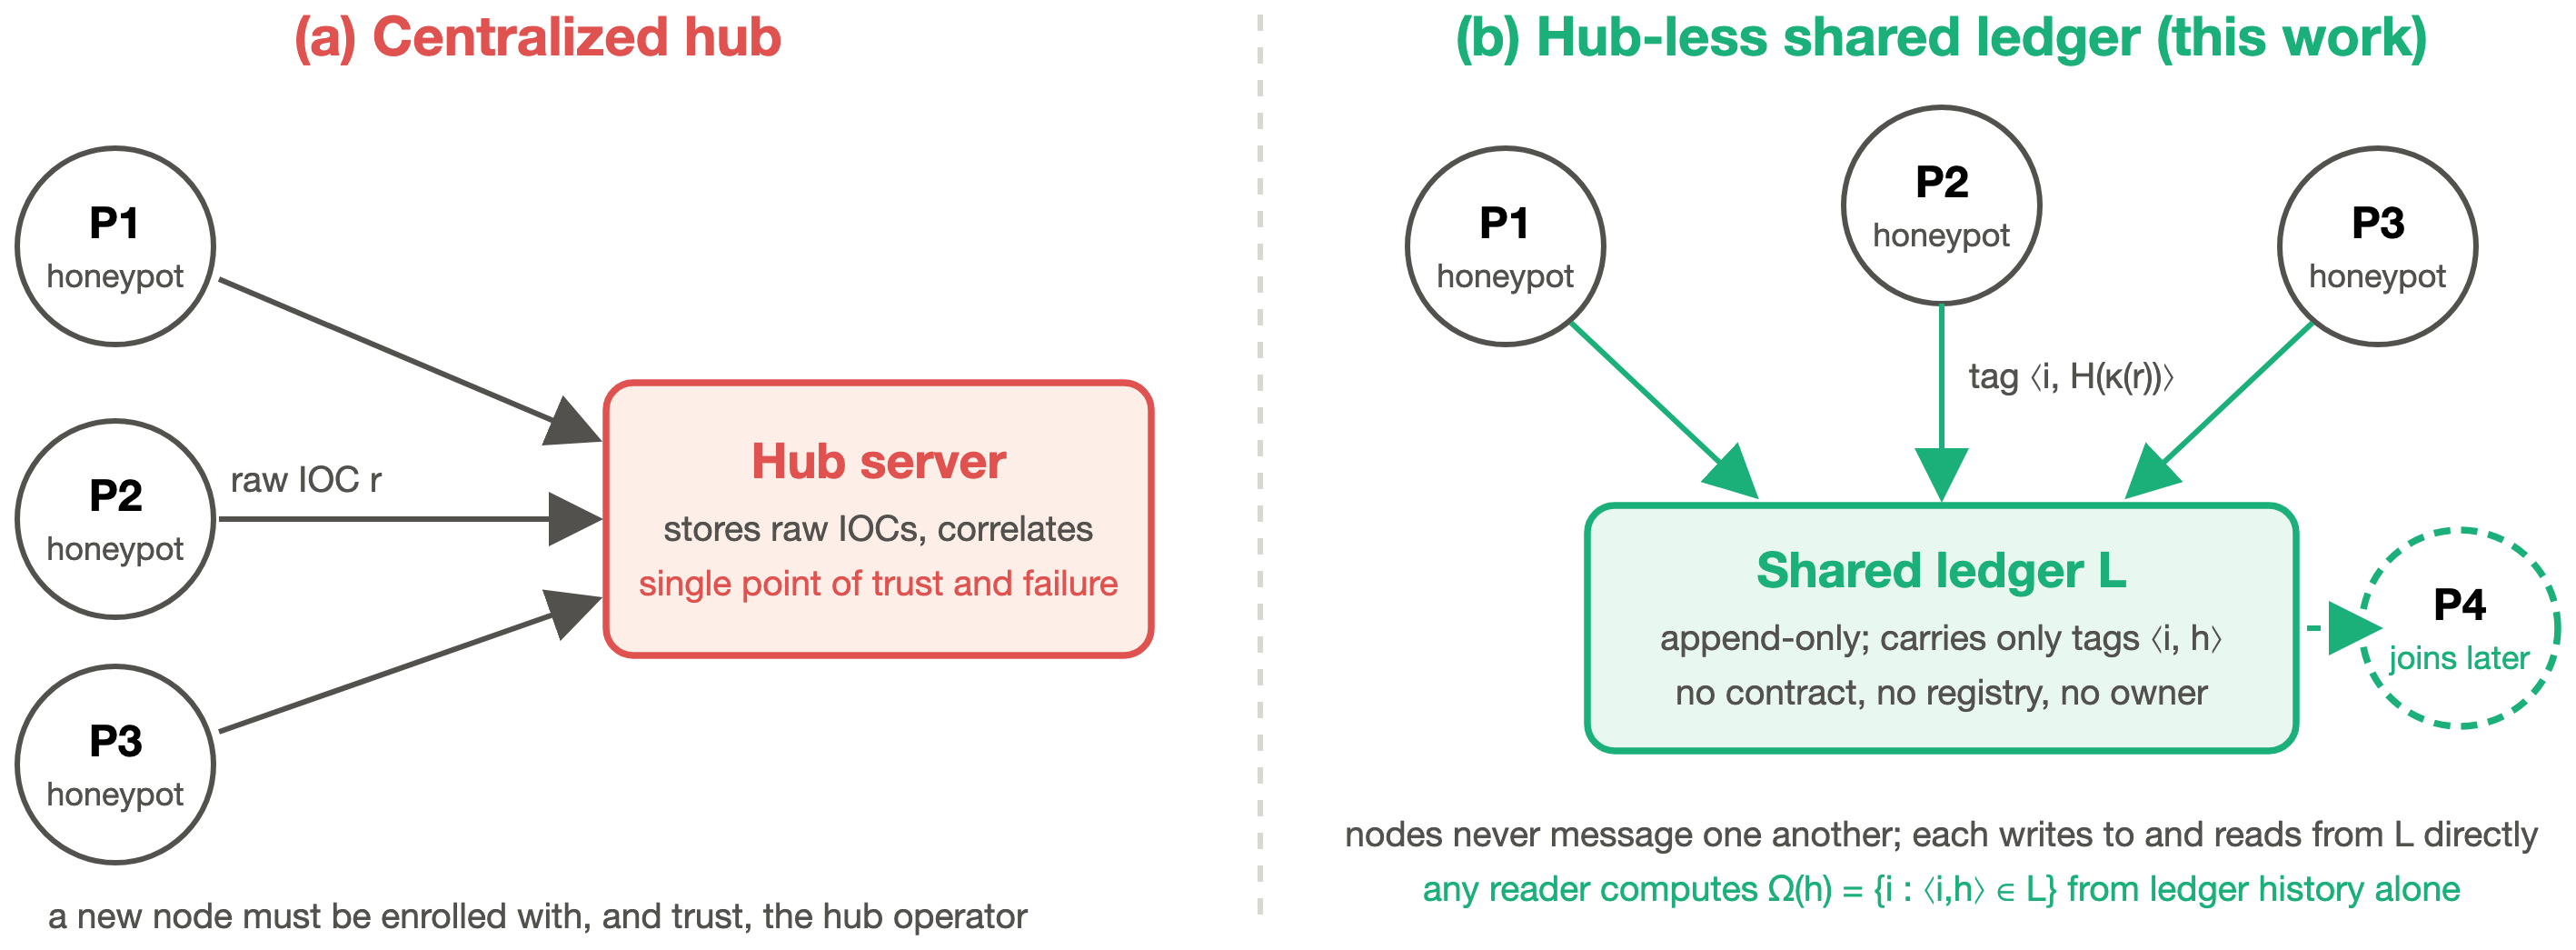
\includegraphics[width=\textwidth]{figures/diag_hubcompare.png}
\caption{System models. (a) Centralized hub: every node sends raw IOCs to one administered server that performs correlation. (b) Hub-less scheme: every node anchors tags $\langle i, H(\kappa(r))\rangle$ to a shared ledger, nodes never communicate, and any reader, including a node that joins later, computes the observer map $\Omega$ from ledger history alone.}
\label{fig:arch}
\end{figure*}

\subsection{Anchoring and reconstruction}
Fig.~\ref{fig:arch} contrasts the two models. Algorithm~\ref{alg:anchor} gives the anchoring step and Algorithm~\ref{alg:boot} the reconstruction a fresh node performs. The ledger executes no logic beyond including a transaction; the decoding rule (line~4 of Algorithm~\ref{alg:boot}) is the entire consensus mechanism above the base chain.

\begin{algorithm}[!t]
\caption{Anchor a record (node $P_i$, record $r$, keying function $\kappa$).}
\label{alg:anchor}
\begin{algorithmic}[1]
\State $h \gets H(\kappa(r))$
\State $\tau \gets$ self-transfer from $a_i$ with calldata $\mathrm{enc}(\langle i,h\rangle)$
\State submit $\tau$; wait for receipt; append $(r,h,\mathrm{ht}(\tau))$ to $S_i$
\end{algorithmic}
\end{algorithm}

\begin{algorithm}[!t]
\caption{Bootstrap a fresh node (block range $[b_0,b_1]$, threshold $k$).}
\label{alg:boot}
\begin{algorithmic}[1]
\State $\Obs \gets \emptyset$
\For{$b = b_0$ \textbf{to} $b_1$}
  \For{each transaction $\tau$ in block $b$}
    \If{$\mathrm{dec}(\mathrm{calldata}(\tau)) = \langle i,h\rangle$}
      \State $\Obs(h) \gets \Obs(h)\cup\{i\}$
    \EndIf
  \EndFor
\EndFor
\State \Return $\Obs$, $\{h : |\Obs(h)|\ge k\}$
\end{algorithmic}
\end{algorithm}

\subsection{Keying functions}
\label{sec:keys}
Corroboration under (\ref{eq:corr}) is exact-match on $\kappa(r)$. Because a campaign rarely presents byte-identical indicators to every target, the choice of $\kappa$ determines what the scheme can corroborate. Four functions are evaluated:
\begin{itemize}
\item $\kappa_{\mathrm{exact}}$: canonical JSON of the full record (deterministic key order).
\item $\kappa_{\mathrm{payload}}$: the payload string only.
\item $\kappa_{\mathrm{tmpl}}$: the payload with 8-hex-digit tokens and dotted-quad addresses replaced by a placeholder.
\item $\kappa_{\mathrm{net}}$: the /24 prefix of the source address concatenated with $\kappa_{\mathrm{tmpl}}$.
\end{itemize}
Coarser functions merge more genuinely related observations and also more unrelated ones; Section~\ref{sec:res-acc} quantifies the trade-off.

\subsection{Commit--reveal against the echo adversary}
\label{sec:cr}
Under the plain scheme, A3 succeeds trivially: any digest visible on the ledger can be re-anchored under a second identity, and (\ref{eq:corr}) cannot distinguish an independent observation from a copy. The extension anchors each digest in two steps. Node $P_i$ draws a random salt $s$ and anchors a \emph{commitment}
\begin{equation}
\langle \mathrm{C}, i, c\rangle,\qquad c=H(i\,\|\,s\,\|\,h),
\end{equation}
which reveals nothing about $h$. After a delay it anchors the \emph{reveal} $\langle \mathrm{R}, i, s, h\rangle$. A reader accepts $i$ as an observer of $h$ only if
\begin{equation}
\tau_c=\langle \mathrm{C}, i, H(i\|s\|h)\rangle\in\Ledger \;\wedge\; \mathrm{ht}(\tau_c) < \mathrm{ht}^{*}(h),
\label{eq:cr}
\end{equation}
where $\mathrm{ht}^{*}(h)=\min_j \mathrm{ht}(\langle \mathrm{R}, j, \cdot, h\rangle)$ is the height of the earliest reveal of $h$ by any node; that is, the commitment must precede every reveal. An echo adversary learns $h$ only from a reveal, so its commitment cannot satisfy (\ref{eq:cr}). The cost is two transactions per IOC and a bounded corroboration window: an honest node that first observes $h$ after another node has already revealed it is also rejected by (\ref{eq:cr}). Algorithm~\ref{alg:cr} gives the validation rule.

\emph{Epoch workflow and late observations.} A deployment divides time into epochs of fixed length $\Delta$. Within epoch $e$ each node commits every digest observed since its last commit; commitments close at the epoch boundary, after which the nodes anchor the corresponding reveals. Rule~(\ref{eq:cr}) is evaluated per epoch, so a commitment in $e$ competes only with reveals in $e$, and an observation arriving after the reveal phase is not discarded: the node holds it and commits it in $e+1$, corroborating with any node that also observed it in that window. Nodes observing $h$ in different epochs are recorded as observers in those epochs, so a reader requiring corroboration within one epoch counts them separately, while a reader that unions the per-epoch observer sets counts them together at the cost of admitting an adversary that echoes across a boundary. Corroboration of a campaign straddling a boundary is thus delayed by at most one epoch under the union rule and lost under the strict rule, making $\Delta$ the parameter that trades detection latency against echo resistance. Section~\ref{sec:res-adv} measures the strict rule in a single epoch, the conservative case; the recall cost of a given $\Delta$ depends on campaign duration and is not measured here (Section~\ref{sec:cr-window}).

\begin{algorithm}[!t]
\caption{Validate commit--reveal anchors (block range $[b_0,b_1]$).}
\label{alg:cr}
\begin{algorithmic}[1]
\State $\mathit{Com}\gets\emptyset$; $\mathit{Rev}\gets[\,]$
\For{each $\tau$ in blocks $b_0..b_1$}
  \If{$\mathrm{dec}(\tau)=\langle\mathrm{C},i,c\rangle$}
    \State $\mathit{Com}[(i,c)]\gets\min(\mathit{Com}[(i,c)],\mathrm{ht}(\tau))$
  \ElsIf{$\mathrm{dec}(\tau)=\langle\mathrm{R},i,s,h\rangle$}
    \State append $(\mathrm{ht}(\tau),i,s,h)$ to $\mathit{Rev}$
  \EndIf
\EndFor
\State $\mathrm{ht}^{*}[h]\gets\min\{b:(b,\cdot,\cdot,h)\in\mathit{Rev}\}$ for each $h$
\For{each $(b,i,s,h)\in\mathit{Rev}$}
  \State $c\gets H(i\|s\|h)$
  \If{$(i,c)\in\mathit{Com}$ \textbf{and} $\mathit{Com}[(i,c)]<\mathrm{ht}^{*}[h]$}
    \State $\Obs(h)\gets\Obs(h)\cup\{i\}$
  \EndIf
\EndFor
\end{algorithmic}
\end{algorithm}

\section{Experimental Setup}
\label{sec:setup}

\subsection{Testbed}
All experiments run against Ganache 7.9.2~\cite{ref19} (chain id 1337), an Ethereum-compatible development chain that includes each transaction in its own block immediately, with 24 unlocked accounts so that every writer node and every adversarial identity has its own account and no two writers serialize on a nonce. Nodes are threads in one Python process that communicate with the chain over JSON-RPC on the loopback interface; they share no state and hold no reference to one another. The measured RPC round-trip floor (\texttt{eth\_blockNumber}, $n=200$) is 1.55\,ms mean, 2.10\,ms p95. One harness (\texttt{benchmark\_federation.py}) produces every number in this paper in a single run of 183\,s that mined 13,810 blocks; Table~\ref{tab:params} lists the parameters. The harness, the raw results file and the build scripts are available from the authors.

\begin{table}[!t]
\caption{Parameters of experiments E1--E8.}
\label{tab:params}
\centering
\scriptsize
\setlength{\tabcolsep}{3pt}
\begin{tabular}{@{}lp{0.62\columnwidth}@{}}
\toprule
Exp. & Parameters \\
\midrule
E1 & $N\in\{1,2,4,8,16\}$ writers; 40 events per node; 5 repetitions \\
E2 & ASCII and binary tags, 50 anchors each; $B\in\{1,\dots,64\}$, 10 transactions per $B$ \\
E3 & $H\in\{250,500,1000,2000,4000\}$ blocks; 3 runs each \\
E4 & 5 nodes; 60 records per node; 16 campaigns; 5 datasets; 4 keying functions \\
E5 & Sybil $c\in\{1,2,3\}$, $k\in\{2,3,4\}$, 30 fabricated digests; echo against 3 honest nodes \\
E6 & 500 mutated records in 4 classes; 500 unmodified controls \\
E7 & Hub with $N\in\{1,\dots,16\}$ writers, 5 repetitions; outage with 5 nodes $\times$ 100 \\
E8 & 40 propagation trials; 5\,ms poll interval \\
\bottomrule
\end{tabular}
\end{table}

\subsection{Workloads}
IOC payloads are synthetic. E1--E3 and E5--E8 anchor pseudo-random digests, since only the anchoring mechanics are exercised.

E4 requires labeled ground truth and is constructed as follows. A campaign $c$ is a tuple $(\mathit{tmpl}_c, \mathit{pre}_c, \mathit{tok}_c, \mathit{host}_c, T_c, m_c)$: a payload template from eight hostile command patterns (shell download-and-execute, SQL injection, wallet RPC calls, reconnaissance), a source /24 prefix, a session token, a host octet, a target set $T_c\subseteq\mathcal{P}$ with $2\le|T_c|\le 5$, and a variation mode $m_c$, the last two drawn uniformly. The observation delivered to node $i\in T_c$ instantiates the template according to $m_c$:
\begin{itemize}
\item \emph{fixed}: token and host are $\mathit{tok}_c$ and $\mathit{host}_c$ for every target, so all targets receive a byte-identical record;
\item \emph{token}: fresh random token per target, host fixed (one operator, per-session identifiers);
\item \emph{ip}: fresh random host inside $\mathit{pre}_c$ per target, token fixed (one subnet, rotating source);
\item \emph{token+ip}: both vary;
\item \emph{net}: fresh random /24 per target, token fixed (a distributed botnet).
\end{itemize}
Each record carries its campaign identifier and noise records carry $\bot$; these labels are the ground truth for Section~\ref{sec:metrics} and are never visible to the reconstruction, which sees only anchored digests. 16 campaigns are generated per dataset, and each node's stream is filled to 60 records with noise: generic commands (\texttt{cat /etc/passwd}, \texttt{id}, \texttt{GET /.env}) from random addresses, which unrelated attackers also produce and which therefore collide across nodes under coarse keys. The modes span the range from a byte-identical indicator to one sharing only a command template; they are not a claim about how often each occurs in the wild (Section~\ref{sec:validity}).

\subsection{Metrics}
\label{sec:metrics}
Latency is the wall-clock time from submitting a transaction to receiving its receipt. Throughput is confirmed events divided by the wall-clock time of the concurrent run. Gas is the \texttt{gasUsed} field of the receipt. Corroboration accuracy is scored at campaign level: a corroborated key is a true positive if every observation under it belongs to one campaign, and a false positive if it merges observations from different campaigns or from noise; a multi-target campaign with no true-positive key is a false negative. Precision, recall and $F_1$ follow. Confidence intervals are $1.96\,\sigma/\sqrt{n}$ over repetitions. Tamper detection succeeds when the original tag is present under the victim's identity and the forged digest is absent; an unmodified control is a false positive if (\ref{eq:consistent}) fails for it.

\subsection{Centralized baseline}
The hub is an in-process HTTP server with a mutex-protected in-memory list. The same writer counts post the same IOC volume to it, using the same thread model, so latency and throughput are directly comparable. For the outage experiment the server is stopped once half of $5\times100$ submissions have been accepted; submissions that fail are counted, as is the number of accepted records that exist only in the hub's memory.

\section{Results}
\label{sec:results}

\subsection{Scaling with the number of writer nodes}
\label{sec:res-scale}
Table~\ref{tab:scaling} and Fig.~\ref{fig:scaling} report E1 and E7. All 6,200 ledger anchors and all hub submissions succeeded. Ledger throughput rises from 119 events/s with one writer to 210 with two and 236 with four, and saturates near 255 events/s from $N=8$ onward; the chain includes transactions serially, so additional writers queue. The median anchor latency is nearly flat (8.12\,ms at $N=1$, 11.74\,ms at $N=16$) but the tail grows once the chain is saturated: p99 reaches 510\,ms at $N=8$ and 1,118\,ms at $N=16$, with a maximum of 2,125\,ms. At $N=1$ the anchor latency of 8.41\,ms comprises roughly two RPC round trips (submit and receipt, 1.55\,ms each) plus inclusion.

The hub sustains 1,478--1,737 events/s with a median of 0.62\,ms at $N=1$, that is, 6.8$\times$ the ledger's saturated throughput at a small fraction of its latency. This is the measured price of removing the intermediary on this testbed; on a distributed chain the gap widens by the consensus term (Section~\ref{sec:discussion}). In the outage run the hub accepted 251 of 500 submissions before being stopped; the remaining 249 were refused, and the 251 accepted records existed only in the stopped process, so no third party could recover them. The equivalent failure for the ledger is loss of the chain itself, which a replicated deployment is designed to prevent; a single Ganache process does not demonstrate that property and we do not claim it from this experiment.

\begin{table}[!t]
\caption{E1 and E7: scaling with the number of concurrent writers (5 repetitions, $\pm$ = 95\% CI).}
\label{tab:scaling}
\centering
\scriptsize
\setlength{\tabcolsep}{3pt}
\begin{tabular}{@{}rrrrrrrr@{}}
\toprule
& \multicolumn{5}{c}{Shared ledger} & \multicolumn{2}{c}{Central hub} \\
\cmidrule(lr){2-6}\cmidrule(lr){7-8}
$N$ & events/s & med.\ ms & p95 ms & p99 ms & max ms & events/s & med.\ ms \\
\midrule
1 & 119.2 $\pm$ 8.0 & 8.12 & 9.8 & 12 & 52 & 1478 $\pm$ 248 & 0.62 \\
2 & 209.5 $\pm$ 4.9 & 9.38 & 11.0 & 12 & 15 & 1660 $\pm$ 280 & 1.11 \\
4 & 236.4 $\pm$ 5.3 & 11.03 & 24.9 & 60 & 133 & 1692 $\pm$ 153 & 2.23 \\
8 & 253.4 $\pm$ 4.9 & 11.19 & 33.6 & 510 & 850 & 1712 $\pm$ 92 & 3.59 \\
16 & 255.0 $\pm$ 2.9 & 11.74 & 45.0 & 1118 & 2125 & 1737 $\pm$ 42 & 3.76 \\
\bottomrule
\end{tabular}
\end{table}

\begin{figure}[!t]
\centering
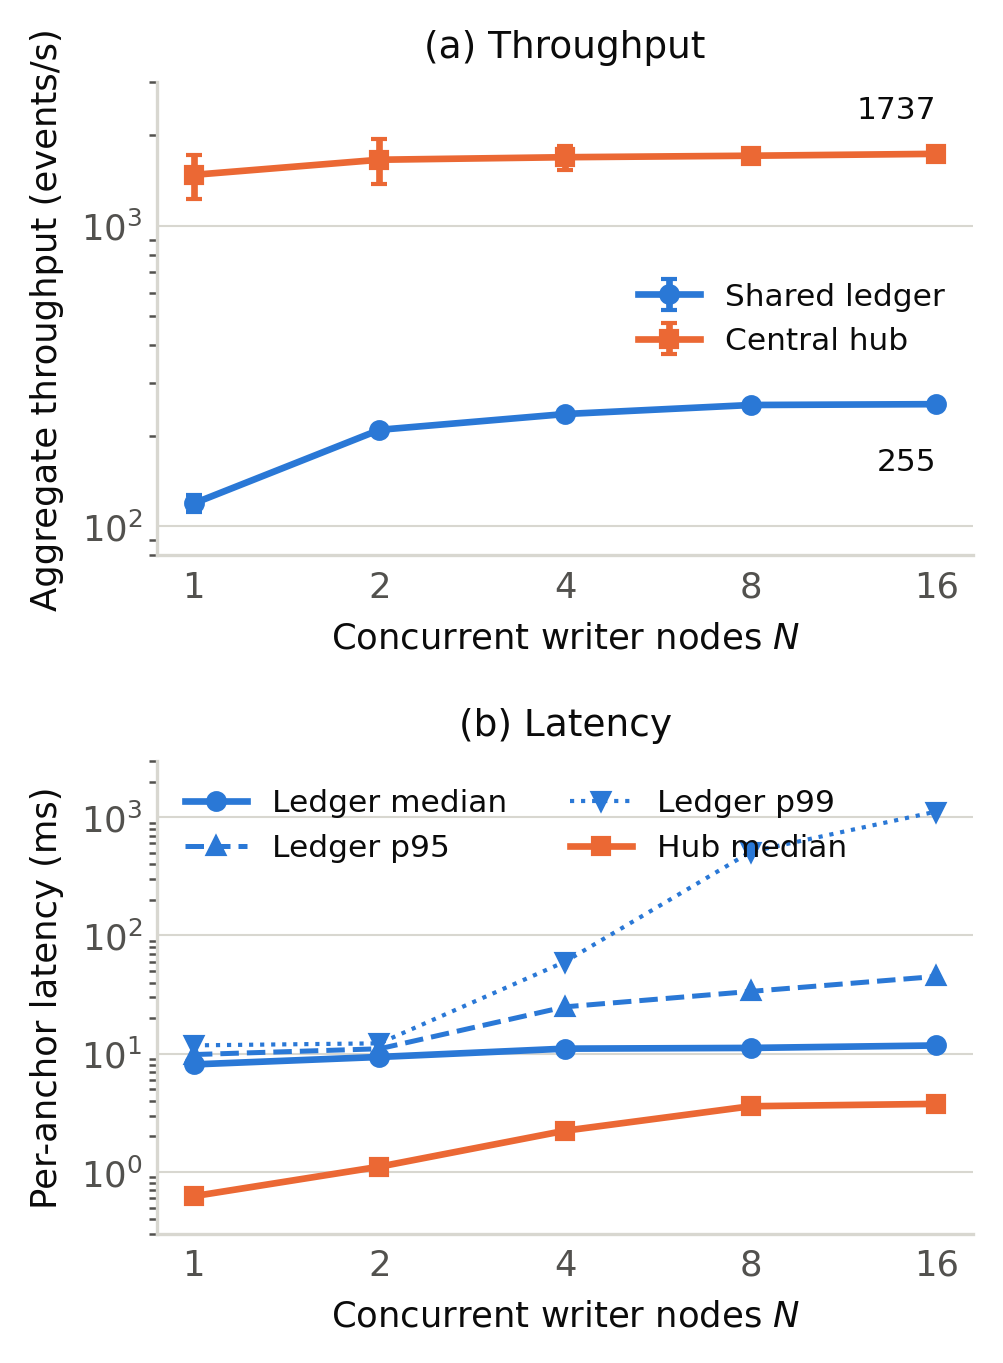
\includegraphics[width=0.95\columnwidth]{figures/fig_scaling.png}
\caption{E1 and E7: (a) aggregate throughput and (b) per-event latency versus the number of concurrent writer nodes, for the shared ledger and the centralized hub, both measured in the same harness. Error bars in (a) are 95\% confidence intervals over 5 repetitions. Axes are logarithmic.}
\label{fig:scaling}
\end{figure}

\subsection{Gas cost, encoding and batching}
Table~\ref{tab:gas} reports E2. Measured gas equals the EIP-2028 model (\ref{eq:gas}) to the unit for both encodings: 22,120 for the 70-byte ASCII tag and 21,545 for the 35-byte binary tag, a saving of 2.6\%. The intrinsic 21,000 gas dominates; calldata contributes only 1,120 gas even for the ASCII tag, so shrinking the tag has limited effect and batching is the lever that matters. With $B$ digests per transaction the gas per IOC falls as $g/B$ (Fig.~\ref{fig:batching}), from 21,552 at $B=1$ to 337 at $B=64$; per-transaction gas is constant at 21,554 because the root is 32 bytes regardless of $B$. All 1,270 membership proofs verified, and proof size grows as $32\lceil\log_2 B\rceil$ bytes, from 0 at $B=1$ to 192 bytes at $B=64$. Per-IOC latency falls proportionally, from 8.72\,ms to 0.12\,ms, at the cost of holding IOCs until a batch fills.

\begin{table}[!t]
\caption{E2 and E5: measured gas per anchored IOC.}
\label{tab:gas}
\centering
\scriptsize
\setlength{\tabcolsep}{3pt}
\begin{tabular}{@{}lrrrr@{}}
\toprule
Scheme & Bytes & Gas/tx & Gas/IOC & Eq.~(\ref{eq:gas}) \\
\midrule
ASCII tag, $B=1$ & 70 & 22,120 & 22,120 & 22,120 \\
Binary tag, $B=1$ & 35 & 21,545 & 21,545 & 21,545 \\
Merkle root, $B=8$ & 37 & 21,554 & 2,694 & -- \\
Merkle root, $B=64$ & 37 & 21,554 & 337 & -- \\
Commit + reveal, $B=1$ & 40 + 89 & 21,638 + 22,424 & 44,062 & -- \\
\bottomrule
\end{tabular}
\end{table}

\begin{figure}[!t]
\centering
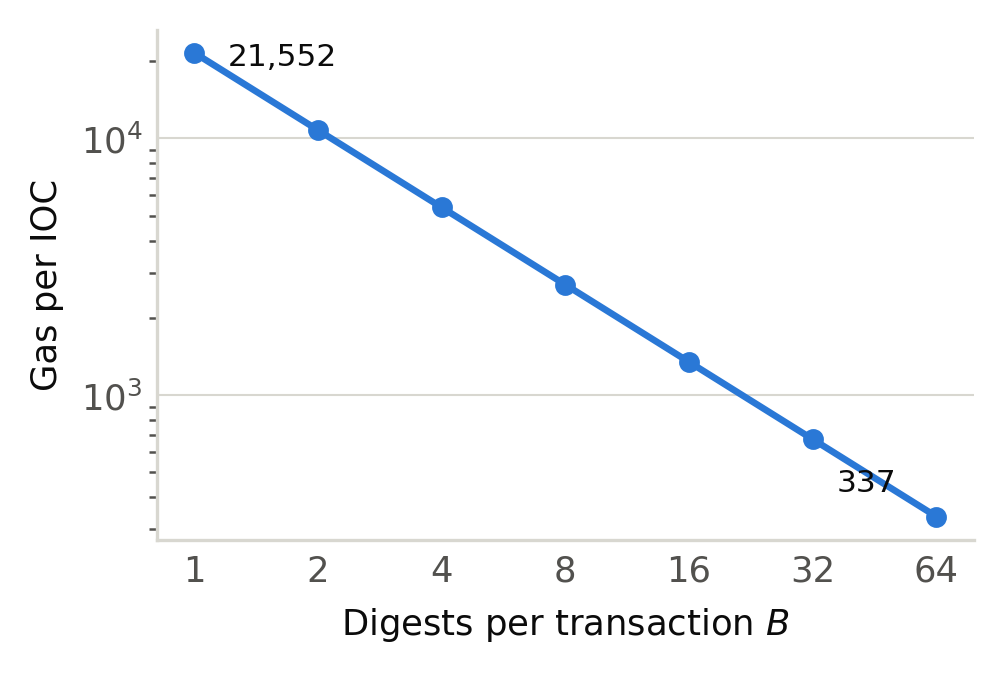
\includegraphics[width=0.9\columnwidth]{figures/fig_batching.png}
\caption{E2: measured gas per IOC versus digests per transaction $B$ (10 transactions per point; all 1,270 membership proofs verified).}
\label{fig:batching}
\end{figure}

\subsection{Bootstrap cost}
Fig.~\ref{fig:bootstrap} reports E3. Reconstruction time is linear in history length with $\beta=3.01$\,ms per block and $R^2=0.998$; scanning 4,000 blocks takes 12.0\,s. The per-block cost is about twice the RPC floor, the remainder being JSON decoding of a full block with transaction bodies. Since the chain includes one anchor per block, this is also the per-anchor bootstrap cost; on a chain that packs many anchors per block the per-anchor cost is lower by the packing factor. A node that has been offline can resume from its last scanned height rather than from genesis.

\begin{figure}[!t]
\centering
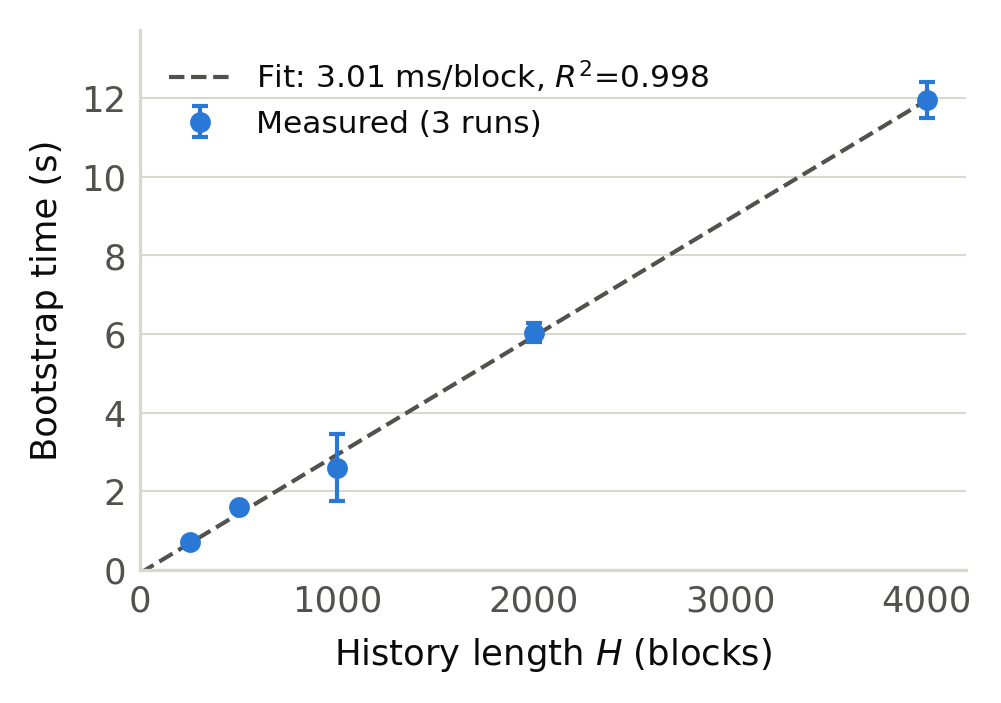
\includegraphics[width=0.9\columnwidth]{figures/fig_bootstrap.png}
\caption{E3: time for a fresh node to rebuild the observer map from $H$ blocks of history (mean of 3 runs, 95\% CI), with the least-squares fit of (\ref{eq:boot}).}
\label{fig:bootstrap}
\end{figure}

\subsection{Corroboration accuracy under per-target variation}
\label{sec:res-acc}
Table~\ref{tab:acc} and Fig.~\ref{fig:accuracy} report E4 over 5 datasets (6,000 anchors in total, reconstructed from the chain for every keying function). Exact-record hashing has perfect precision but recovers only 27.5\% of multi-target campaigns, because it corroborates only the \emph{fixed} mode. Payload-only hashing raises recall to 66.2\% but precision falls to 56.4\%: generic noise commands from unrelated attackers collide across nodes and are reported as campaigns. The template key attains the lowest precision and the lowest recall of the four (F$_1$ = 0.15) because stripping tokens and addresses makes distinct campaigns that share a tool indistinguishable. The /24+template key is best (precision 100\%, recall 81.2\%, F$_1$ = 0.89); its misses are the \emph{net} campaigns, whose sources span unrelated prefixes and which no address-based key can join. No single keying function is adequate for every campaign shape.

\begin{table}[!t]
\caption{E4: campaign-level corroboration accuracy by keying function (5 datasets, $\pm$ = 95\% CI; TP/FP/FN summed).}
\label{tab:acc}
\centering
\footnotesize
\begin{tabular}{@{}lccccc@{}}
\toprule
$\kappa$ & Precision & Recall & $F_1$ & TP/FP/FN \\
\midrule
$\kappa_{\mathrm{exact}}$ & 1.000 $\pm$ 0.000 & 0.275 $\pm$ 0.083 & 0.424 $\pm$ 0.109 & 22/0/58 \\
$\kappa_{\mathrm{payload}}$ & 0.564 $\pm$ 0.044 & 0.662 $\pm$ 0.138 & 0.607 $\pm$ 0.082 & 53/40/27 \\
$\kappa_{\mathrm{tmpl}}$ & 0.154 $\pm$ 0.060 & 0.150 $\pm$ 0.062 & 0.152 $\pm$ 0.061 & 12/65/68 \\
$\kappa_{\mathrm{net}}$ & 1.000 $\pm$ 0.000 & 0.812 $\pm$ 0.129 & 0.890 $\pm$ 0.086 & 65/0/15 \\
\bottomrule
\end{tabular}
\end{table}

\begin{figure}[!t]
\centering
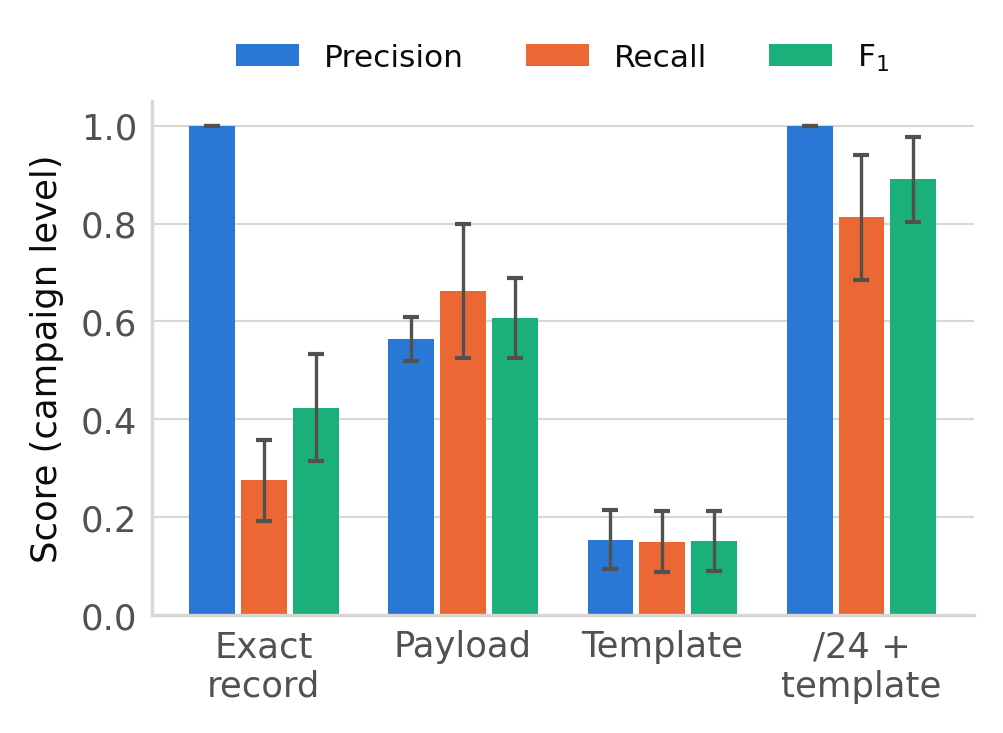
\includegraphics[width=0.95\columnwidth]{figures/fig_accuracy.png}
\caption{E4: precision, recall and $F_1$ of campaign-level corroboration for the four keying functions (95\% CI over 5 datasets).}
\label{fig:accuracy}
\end{figure}

\subsection{Adversarial writers}
\label{sec:res-adv}
Table~\ref{tab:adv} reports E5. Against A2, a fabricated digest satisfies $C_k$ exactly when the adversary controls $c\ge k$ identities: with $c=1$ none of 30 fabricated digests reach $k=2$; with $c=2$ all reach $k=2$ and none reach $k=3$; with $c=3$ all reach $k=3$ and none reach $k=4$. The threshold therefore expresses a bound on the number of Sybil identities tolerated rather than a defense against them, and is meaningful only where identity creation carries a cost, as on a permissioned or stake-weighted chain.

Against A3 the plain scheme offers no resistance. After three honest nodes anchored 120 distinct digests, an echo node read the ledger and re-anchored all of them in 1.04\,s; every one of the 120 single-observer digests then satisfied $C_2$. Under commit--reveal, with two honest nodes sharing 20 digests and three nodes holding 90 private ones, the echo node's 110 reveals were all rejected by (\ref{eq:cr}), no private digest was falsely corroborated, and all 20 genuinely shared digests were still corroborated. The cost is 44,062 gas per IOC (2.0$\times$ the single-tag cost) and two inclusion latencies (9.0 and 8.3\,ms mean).

\begin{table}[!t]
\caption{E5: adversarial writers.}
\label{tab:adv}
\centering
\footnotesize
\begin{tabular}{@{}lrrrr@{}}
\toprule
\multicolumn{5}{@{}l}{(a) Sybil: fabricated digests (of 30) satisfying $C_k$} \\
Identities $c$ & & $k=2$ & $k=3$ & $k=4$ \\
\midrule
1 & & 0 & 0 & 0 \\
2 & & 30 & 0 & 0 \\
3 & & 30 & 30 & 0 \\
\midrule
\multicolumn{5}{@{}l}{(b) Echo: single-observer digests falsely satisfying $C_2$} \\
Scheme & Single-obs. & False & Rate & Gas/IOC \\
\midrule
Plain tag & 120 & 120 & 100\% & 22,120 \\
Commit--reveal & 90 & 0 & 0\% & 44,062 \\
\bottomrule
\end{tabular}
\end{table}

\subsection{Tamper detection}
In E6, 500 anchored records were each mutated in one of four ways (payload suffix, source address change, field deletion, single-bit flip in the payload) and checked against (\ref{eq:consistent}); 500 of 500 were detected, 125 of 125 in each class. All 500 unmodified controls passed, giving a false-positive rate of 0. The check costs 9.6\,$\mu$s per record once $\Obs$ is in memory. The result follows from the collision resistance of $H$ and the immutability of included transactions; the experiment establishes that the encoding, decoding and lookup path preserve those properties end to end, including the provenance component of (\ref{eq:consistent}).

\subsection{Propagation to an independent reader}
In E8 a reader with no channel to the writer polled the chain at 5\,ms intervals and observed each of 40 anchors after a mean of 2.07\,ms (p95 3.21\,ms) from inclusion. On this testbed the figure is the polling loop's reaction time and contains no network or consensus delay; it is a lower bound.

\section{Discussion and Limitations}
\label{sec:discussion}

\subsection{What transfers from a local chain}
\label{sec:transfer}
The chain includes each transaction immediately and in its own block, so no measurement here contains block time, consensus latency or gossip delay. On a public or consortium chain, anchor latency and propagation acquire a term of seconds to tens of seconds, and throughput is bounded by the chain's block gas limit rather than by the 255 events/s serialization point observed here. What transfers unchanged are the gas model, the $g/B$ batching law and proof sizes, the linear bootstrap cost per block, the accuracy trade-off among keying functions, the Sybil bound and the commit--reveal argument, none of which depends on block production. The scaling shape transfers in kind: a single ordering point saturates and pushes latency into the tail.

\subsection{Identity and Sybil resistance}
The scheme assumes one node per account, so on a permissionless chain, where accounts are free, A2 succeeds for any $k$. The intended deployment is a consortium chain, or a public chain with an out-of-band allowlist of node keys, where identity creation is administered. This reintroduces an enrollment step, but a one-time one that is not on the data path.

\subsection{Commit--reveal window}
\label{sec:cr-window}
Rule~(\ref{eq:cr}) rejects any observer whose commitment follows the first reveal of $h$, including honest late observers. The epoch schedule of Section~\ref{sec:cr} bounds that loss to observations straddling a boundary, which a node re-commits in the next epoch; the resulting recall cost depends on campaign duration relative to $\Delta$ and is not measured here.

\subsection{Gas at scale}
Every anchor is a paid transaction, and on-chain cost grows with the number of nodes and their observation rates, whereas a hub pays nothing per record. Batching reduces the per-IOC cost by $B$; at $B=64$ it is 337 gas, about 1.6\% of a bare transfer, and the trade is immediacy. Whether this is acceptable depends on the fee level of the chosen chain and is a deployment decision outside this paper.

\subsection{Threats to validity}
\label{sec:validity}
We state the scope of each measurement explicitly.
\emph{Synthetic corroboration workload.} The E4 dataset is generated rather than captured: 16 campaigns per dataset over five variation modes, 5 datasets. It supplies the campaign labels that precision and recall require and captured traffic does not, but it does not reproduce the diversity of real attack traffic, so Table~\ref{tab:acc} characterizes this workload rather than a deployment. What the experiment establishes is the mechanism and its ordering: an exact-match key corroborates no campaign that varies per target, and each relaxation recovers some campaigns while merging some unrelated ones. That ordering follows from the definitions of the keys and modes, not from the sample size.

\emph{Sensitivity of the keying functions.} The keys were fixed before the datasets were generated, but their normalization rules (8-hex-digit tokens, dotted-quad addresses, /24 prefixes) match the structure of the generated variation, so their measured accuracy upper-bounds what those rules achieve against unseen variation such as encoded payloads, padded commands or per-target reordering. We neither tuned the keys nor evaluated them outside the five modes; a deployment should measure its own key against its own traffic. The ledger is neutral on that choice, which is the property the experiment is designed to show: the same anchored evidence supports any $\kappa$, and a node may anchor under several.

\emph{Scale of the adversarial evaluation.} E5 exercises 30 fabricated digests under $c\in\{1,2,3\}$ identities and one echo adversary. The Sybil result verifies the arithmetic of~(\ref{eq:corr}), that $c$ identities satisfy $C_k$ exactly when $c\ge k$, which holds for any $c$; a larger trial would add only the cost of acquiring identities on a given chain, a property of its admission policy rather than of the scheme. Neither adversary is adaptive: we model no attacker that observes the corroboration output and adjusts its anchoring, nor one that times reveals to exploit epoch boundaries.

\emph{Absence of real consensus.} Ganache mines each transaction immediately into its own block, so the 255 events/s saturation point, the millisecond latencies and the 2.07\,ms propagation figure contain no block time, consensus round, gossip propagation or reorganization behavior; they characterize the software above the chain. Section~\ref{sec:transfer} lists the results independent of block production: the throughput and latency figures are not among them and must be read with the chosen chain's consensus term added.

\emph{Remaining items.} Nodes are threads in one process, so interpreter and loopback contention inflate the tail latencies at $N\ge 8$. The hub baseline is a minimal in-memory server: a production platform would be slower per request but would still pay no per-record transaction cost. The commit--reveal recall cost per epoch length is unmeasured (Section~\ref{sec:cr-window}).

\section{Conclusion}
A shared ledger carrying nothing but tagged hashes can replace the correlation function of a central threat-intelligence hub for a set of honeypots that do not trust one another. Measured on a live chain with up to 16 writers, the scheme serializes at about 255 events/s, costs 22,120 gas per IOC unbatched and 337 gas at $B=64$, exactly as the calldata model predicts, and lets a new node rebuild the global view at 3.01\,ms per block. The accuracy of the corroboration signal depends on the keying function: exact hashing recovers 27.5\% of varied campaigns, a /24-plus-template key recovers 81.2\% at full precision, and coarser keys trade precision for recall. The plain scheme is defenseless against an echo adversary; a commit--reveal extension removes that attack at 2.0$\times$ the gas and a bounded corroboration window. Against a measured hub the ledger costs a factor of 6.8 in throughput on this testbed and more on a distributed chain. These are the measured costs of removing the trusted intermediary.

{\footnotesize
\begin{thebibliography}{00}
\setlength{\itemsep}{0pt plus 0.3pt}
\bibitem{ref1} C. Wagner, A. Dulaunoy, G. Wagener, and A. Iklody, ``MISP: The design and implementation of a collaborative threat intelligence sharing platform,'' in \emph{Proc. ACM Workshop Inf. Sharing Collab. Secur. (WISCS)}, Vienna, Austria, 2016, pp. 49--56.
\bibitem{ref2} OASIS Cyber Threat Intelligence (CTI) Technical Committee, ``STIX Version 2.1,'' OASIS Standard, Jun. 2021. [Online]. Available: \url{https://docs.oasis-open.org/cti/stix/v2.1/stix-v2.1.html}
\bibitem{ref3} OASIS Cyber Threat Intelligence (CTI) Technical Committee, ``TAXII Version 2.1,'' OASIS Standard, Jun. 2021. [Online]. Available: \url{https://docs.oasis-open.org/cti/taxii/v2.1/taxii-v2.1.html}
\bibitem{ref4} C. Ruggiero and S. Bonomi, ``A review of requirements and threats in blockchain-based cyber threat intelligence sharing,'' in \emph{Proc. IEEE 44th Int. Symp. Rel. Distrib. Syst. (SRDS)}, 2025, pp. 410--415, doi: 10.1109/SRDS69199.2025.00050.
\bibitem{ref5} Y. Allouche, N. Tapas, F. Longo, A. Shabtai, and Y. Wolfsthal, ``TRADE: TRusted Anonymous Data Exchange - threat sharing using blockchain technology,'' 2021, \emph{arXiv:2103.13158}.
\bibitem{ref6} H. Ali, W. J. Buchanan, J. Ahmad, M. Abubakar, M. S. Khan, and I. Wadhaj, ``TrustShare: Secure and trusted blockchain framework for threat intelligence sharing,'' \emph{Future Internet}, vol. 17, no. 7, art. 289, 2025, doi: 10.3390/fi17070289.
\bibitem{ref7} K. Dunnett, S. Pal, G. D. Putra, Z. Jadidi, and R. Jurdak, ``A trusted, verifiable and differential cyber threat intelligence sharing framework using blockchain,'' 2022, \emph{arXiv:2208.12031}.
\bibitem{ref8} B. Stojkovski, G. Lenzini, V. Koenig, and S. Rivas, ``What's in a Cyber Threat Intelligence sharing platform? A mixed-methods user experience investigation of MISP,'' in \emph{Proc. 37th Annu. Comput. Secur. Appl. Conf. (ACSAC)}, 2021, pp. 385--398, doi: 10.1145/3485832.3488030.
\bibitem{ref9} T. Jiang, G. Shen, C. Guo, Y. Cui, and B. Xie, ``BFLS: Blockchain and federated learning for sharing threat detection models as cyber threat intelligence,'' \emph{Comput. Netw.}, vol. 224, art. 109604, 2023, doi: 10.1016/j.comnet.2023.109604.
\bibitem{ref10} Y. Otoum, A. Asad, and A. Nayak, ``Blockchain meets adaptive honeypots: A trust-aware approach to next-gen IoT security,'' 2025, \emph{arXiv:2504.16226}.
\bibitem{ref11} K. Dunnett, S. Pal, and Z. Jadidi, ``Challenges and opportunities of blockchain for cyber threat intelligence sharing,'' 2022, \emph{arXiv:2205.03822}.
\bibitem{ref12} A. Tariq, T. Qayyum, S. Alrabaee, and M. A. Serhani, ``Blockchain and distributed ledger technologies for cyberthreat intelligence sharing,'' 2025, \emph{arXiv:2504.02537}.
\bibitem{ref13} L. Lamport, R. Shostak, and M. Pease, ``The Byzantine generals problem,'' \emph{ACM Trans. Program. Lang. Syst.}, vol. 4, no. 3, pp. 382--401, Jul. 1982.
\bibitem{ref14} N. Provos, ``A virtual honeypot framework,'' in \emph{Proc. 13th USENIX Secur. Symp.}, San Diego, CA, USA, 2004, pp. 1--14.
\bibitem{ref15} M. Nawrocki, M. Wahlisch, T. C. Schmidt, C. Keil, and J. Schonfelder, ``A survey on honeypot software and data analysis,'' 2016, \emph{arXiv:1608.06249}.
\bibitem{ref16} A. Vetterl and R. Clayton, ``Bitter Harvest: Systematically fingerprinting low- and medium-interaction honeypots at Internet scale,'' in \emph{Proc. 12th USENIX Workshop Offensive Technol. (WOOT)}, Baltimore, MD, USA, 2018.
\bibitem{ref17} National Institute of Standards and Technology, ``Secure Hash Standard (SHS),'' FIPS PUB 180-4, Aug. 2015.
\bibitem{ref18} G. Wood, ``Ethereum: A secure decentralised generalised transaction ledger,'' Ethereum Project Yellow Paper, 2014.
\bibitem{ref19} Truffle Suite, ``Ganache: A personal Ethereum blockchain for development,'' ConsenSys. [Online]. Available: \url{https://archive.trufflesuite.com/ganache/}
\end{thebibliography}}

\end{document}
